
\section{Current and Future Work: Deep Latent Variable Modeling}

\begin{frame}{Research Direction: Deep Latent-Variable Models for NLP }
  Goal: Expose specific choices as explicit latent variables.   
   \begin{center}
  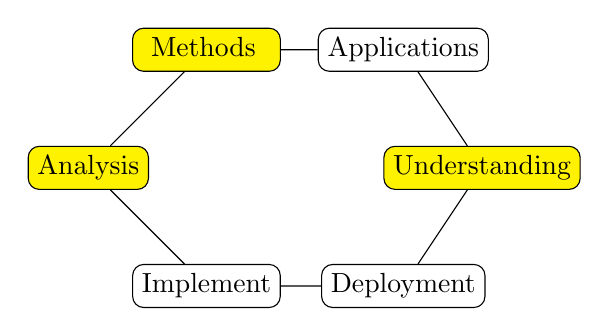
\begin{tikzpicture}
    \node[rounded corners, fill=yellow, draw] (ana) at (-15mm, 15mm) {Analysis};
    \node[rounded corners, fill=yellow,  draw] (meth) at (0mm, 30mm) {\ Methods\phantom{p}};
    \node[rounded corners, draw] (app) at (25mm, 30mm) {Applications};
    \node[rounded corners, fill=yellow, draw] (und) at (35mm, 15mm) {Understanding};
    \node[rounded corners, draw] (dep) at (25mm, 0mm){Deployment};
    \node[rounded corners, draw] (imp) at (0, 0) {Implement};
    \draw (ana) -- (meth) --(app) -- (und) -- (dep) -- (imp) -- (ana);
  \end{tikzpicture}
  \end{center}
\end{frame}

\begin{frame}{Research Direction: \\
      Deep Latent-Variable Models for NLP }

  Goal: Expose specific choices as explicit \textit{discrete} latent variables.


\begin{align*}
p(y, z \param \theta).
\end{align*}

\pause
\begin{itemize}
    \item $y$ is our observed data
    \item $z$ is a collection of problem-specific latent variables
    \item $\theta$ are the deterministic, neural network parameters.
\end{itemize}

% \begin{itemize}
%     \item Data consists of $N$ i.i.d samples,
% \end{itemize}

%                 \[ p(x^{(1:N)}, z^{(1:N)} \param \theta ) = \prod_{n=1}^N p(x^{(n)} \given z^{(n)}; \theta) p(z^{(n)};\theta). \]

\end{frame}

\begin{frame}{Example Model: Mixture of RNNs}

Generative process:
\begin{enumerate}
\item Draw cluster $z \in \{1, \ldots, K\}$ from a Categorical.
\item Draw words $y_{1:T}$ from RNNLM with parameters $\pi_z$.
\end{enumerate}
\[p(y, z \param \theta)
       = \mu_{z} \times   \RNNLM(y_{1:T} \param \pi_z) \]
% \[p(x, z \param \theta)
%       = \mu_{z} \times  \prod_{t=1}^T \softmax(\RNN(\boldh_{t-1}, x_t\param \pi_z))\]
\begin{center}

\begin{tikzpicture}
  %\tikz{
% nodes
\node (dots) {$\ldots$};%
 \node[obs, left=1cm of dots] (x1) {$y_1^{(n)}$};%
 \node[obs, right=1cm of dots] (xT) {$y_T^{(n)}$};%
 \node[latent, above=of dots] (z) {$z^{(n)}$}; %
 \node[const, above=(0.5cm) of z] (mu) {$\mu$};
 \node[const, below left=0.3cm and 0.8cm of x1] (pi) {$\pi$};

% plate
 \plate {plate1} {(dots)(x1)(xT)(z)} {$N$}; %
% edges
 \edge {z} {dots};
 \edge {z} {x1};
 \edge {z} {xT};
 \edge {mu} {z};
 \edge {pi.east} {x1,xT.south};
 \edge {x1} {dots};
 %\edge[bend left] {x1.south} {xT.south};
  \edge {dots} {xT};

 \draw[->]
 (x1) edge[bend right=10] node [right] {} (xT);
 %}
 \end{tikzpicture}
 %}
\end{center}
%\begin{align*}
%\boldh_{z,t} &= \tanh(\mathbf{W}_z \bolde_t +\mathbf{U}_z\boldh_{z,t-1}  + \boldb_{z}) \nonumber \\
%p(x_{t} \given x_{<t} , z) &= \softmax(\mathbf{V} \boldh_{z,t-1} + \boldc)_{x_{t}} \nonumber \\
%p(x_1, \ldots, x_T \given z) &= \prod_{t=1}^{T} p(x_{t} \given x_{<t} , z)
%\end{align*}


\end{frame}


% begin{frame}
% \begin{center}
%     \textbf{ Latent-Variable Model Basics }
%   \end{center}


% \begin{align*}
% p(x, z \param \theta).
% \end{align*}

% \pause
% \begin{itemize}
%     \item $x$ is our observed data
%     \item $z$ is a collection of latent variables
%     \item $\theta$ are the deterministic parameters of the model, such as the neural network parameters
% \end{itemize}

% \pause

% \begin{itemize}
%     \item Data consists of $N$ i.i.d samples,
% \end{itemize}


%                 \[ p(x^{(1:N)}, z^{(1:N)} \param \theta ) = \prod_{n=1}^N p(x^{(n)} \given z^{(n)}; \theta) p(z^{(n)};\theta). \]
% \end{frame}

\begin{frame}{Main Requirement: Posterior Inference}
    For models $p(y, z \param \theta)$, we'll be interested in the \textit{posterior} over latent variables $z$:

    \begin{align*}
        p(z \given y \param \theta) = \frac{\displaystyle p(y, z \param \theta)}{\displaystyle p(y \param \theta)} = \frac{\displaystyle p(y\given z \param  \theta) p(z \param  \theta)}{\displaystyle \sum_{z'} p(y \given z'\param  \theta) p(z'\param  \theta) }.
    \end{align*}

    \air

    \pause
    Why?
    \begin{itemize}
      \item Required for training
      \item Latent $z$ gives separation of data.

% \item Intuition: if I know likely $z^{(n)}$ for $x^{(n)}$, I can learn by maximizing $p(x^{(n)} \given z^{(n)} \param \theta)$.
        % \begin{itemize}
        %     \item Intuition: if I know likely $z^{(n)}$ for $x^{(n)}$, I can learn by maximizing $p(x^{(n)} \given z^{(n)} \param \theta)$.
        % \end{itemize}
    \end{itemize}

    How?

    \begin{itemize}
    \item Sum out over all discrete choices (e.g. run $K$ RNNs).
    \item Variational inference based methods.
    \end{itemize}

\end{frame}


\begin{frame}{ In Applications: Copy-Attention \\
      \small{(Gu et al, 2016) (Gulcehre et al, 2016)}}

Let $z$ be a binary latent variable.
\air
\begin{itemize}
\item If $z = 1$, let the model generate a new word.
\item If $z = 0$, let the model copy a word from the source.
\end{itemize}

Inference:
\begin{center}


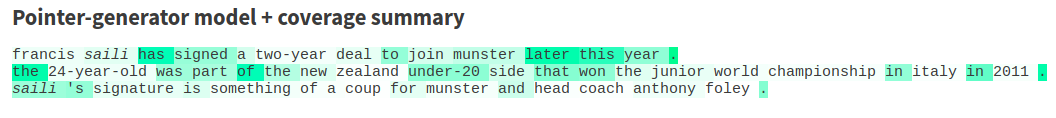
\includegraphics[width=15cm]{seeblog}

\centerline{\small (See et al, 2017)}
\end{center}
\end{frame}


\begin{frame}{ Latent Variable Models for Generation}

  \begin{itemize}
  \item Can we develop other discrete latent-variable models for generation?
    \air
  \item Perhaps each important aspect of generation can be built-in directly.
    \air
  \item Goals:
    \begin{itemize}
    \item Model Control
    \item Model Debugging
    \item Model Uncertainty
    \end{itemize}
  \end{itemize}
\end{frame}





\begin{frame}{Approach 1: Learning Neural Templates}

  \begin{center}
    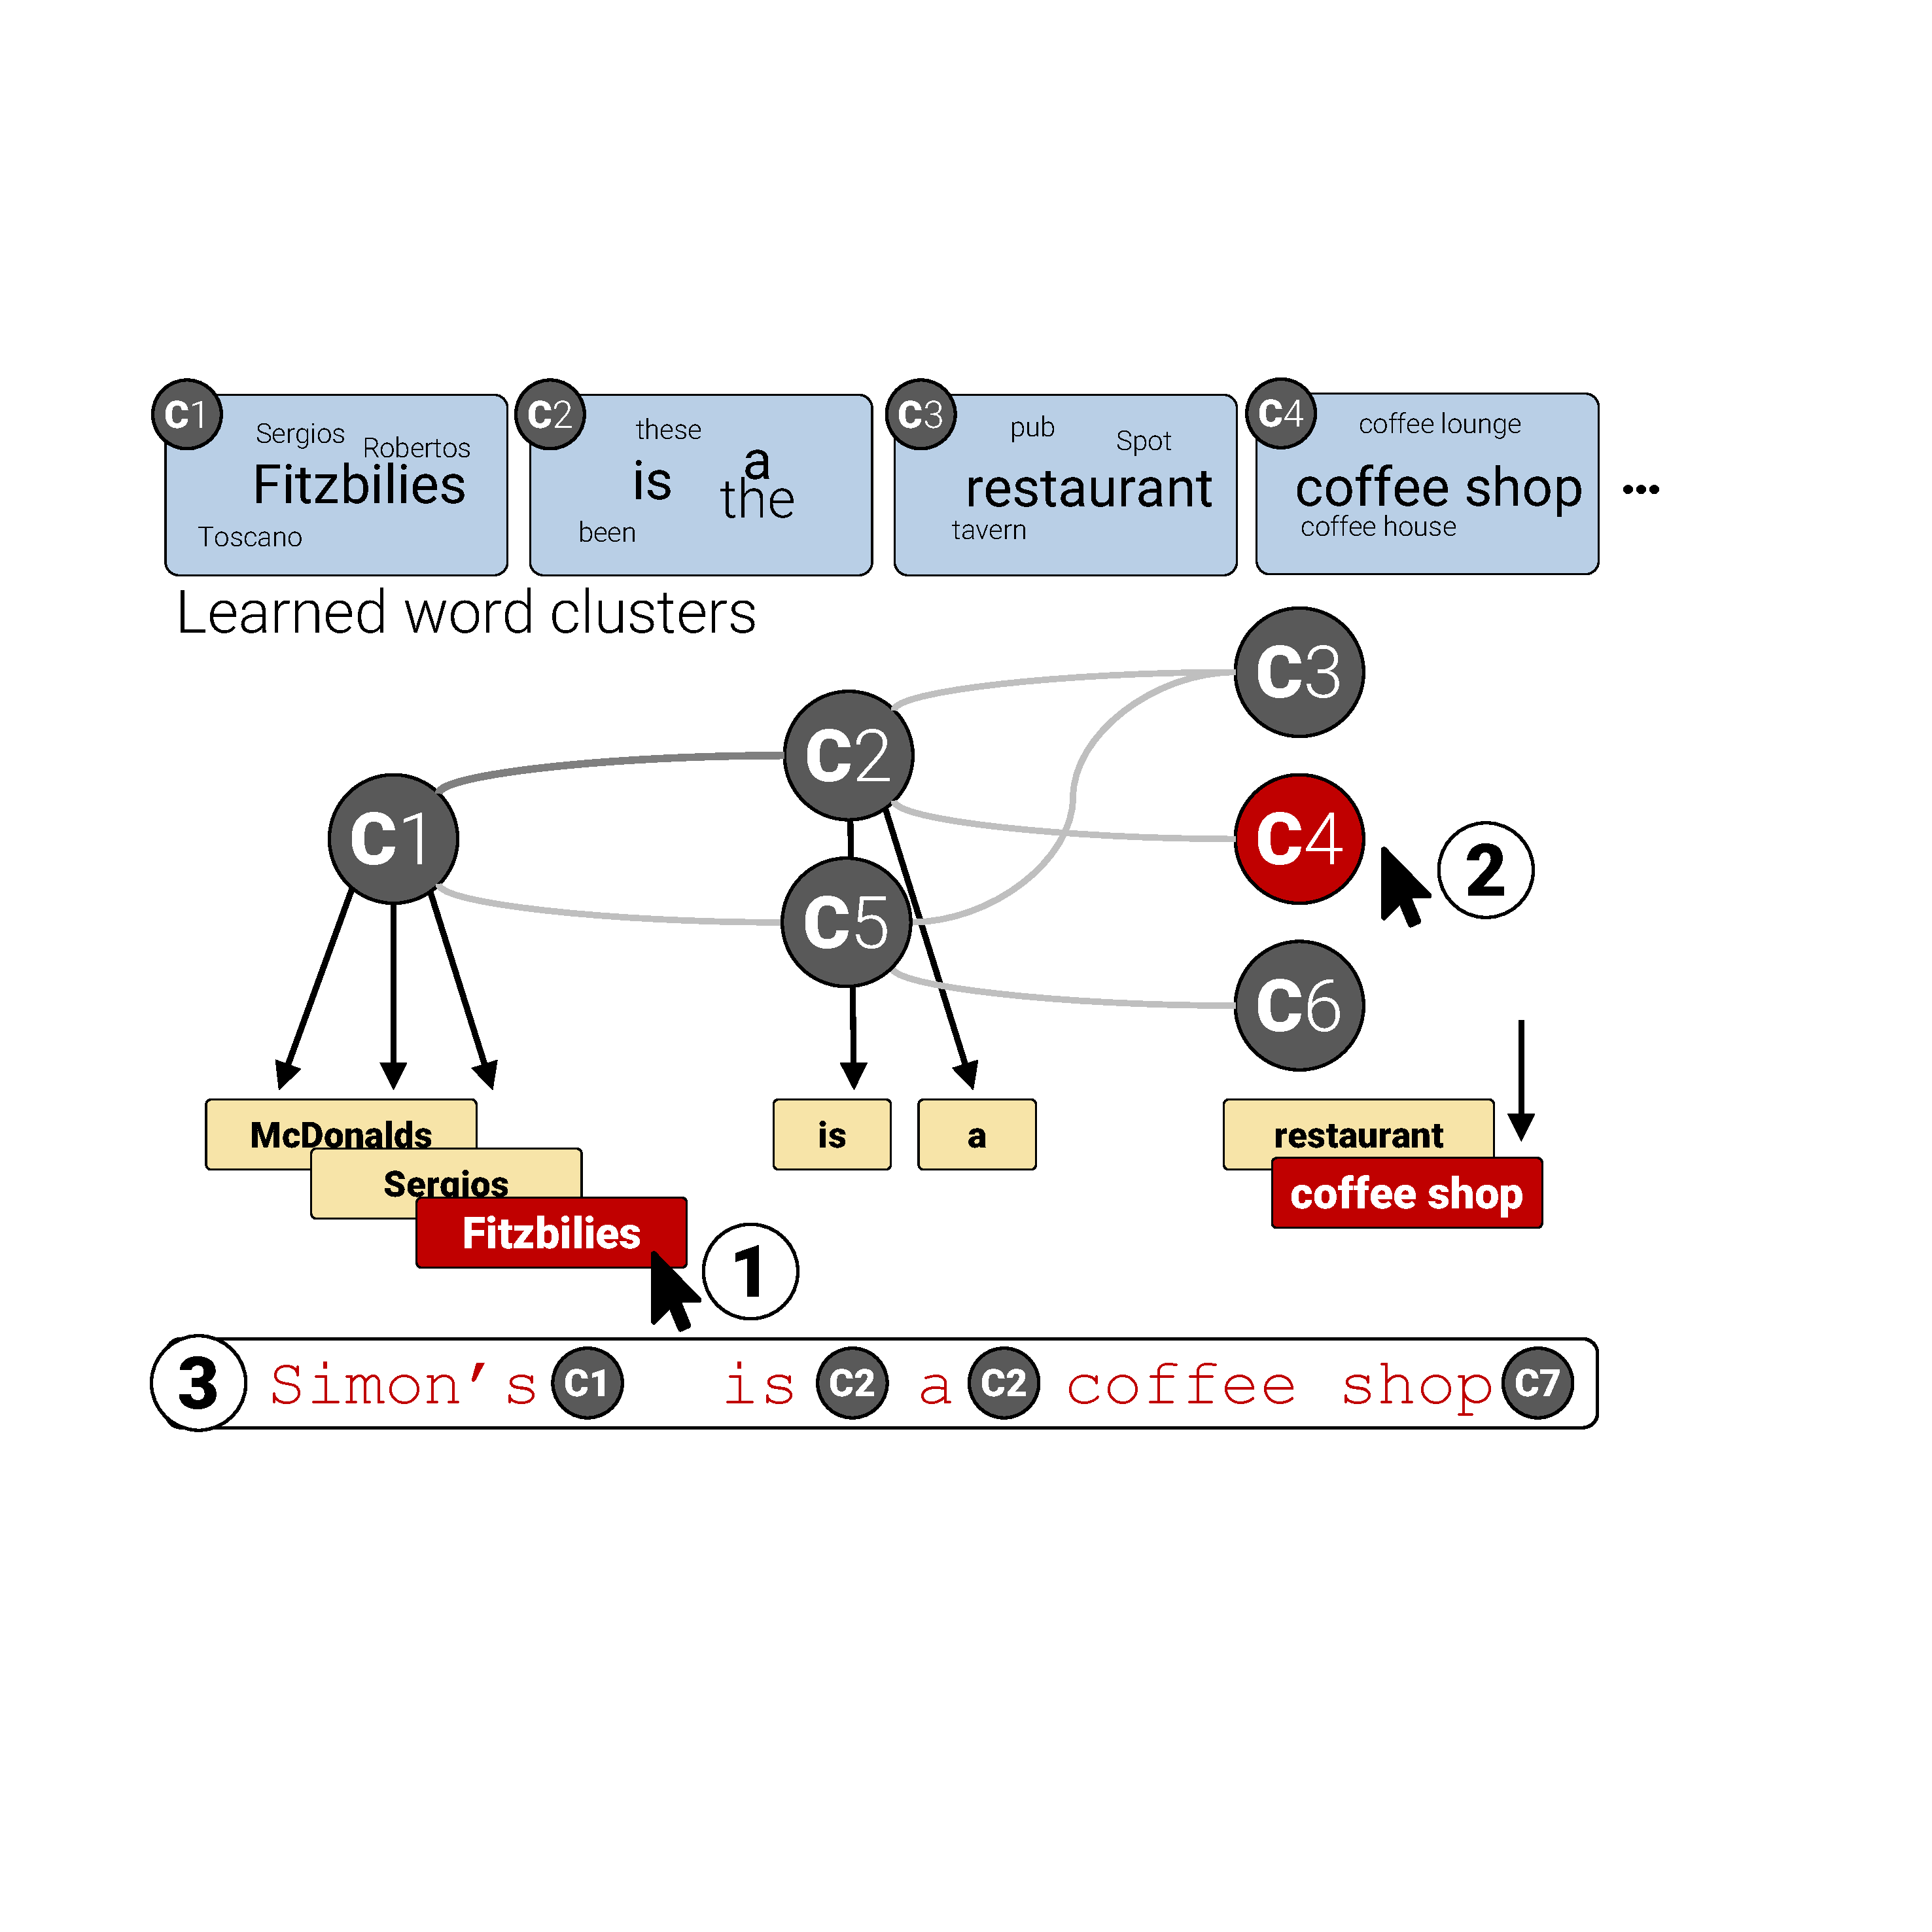
\includegraphics[width=0.7\textwidth]{DecoderVis}
  \end{center}
\end{frame}

\begin{frame}{Approach 2: Latent Alignment and Variational Attention}
  \begin{center}
    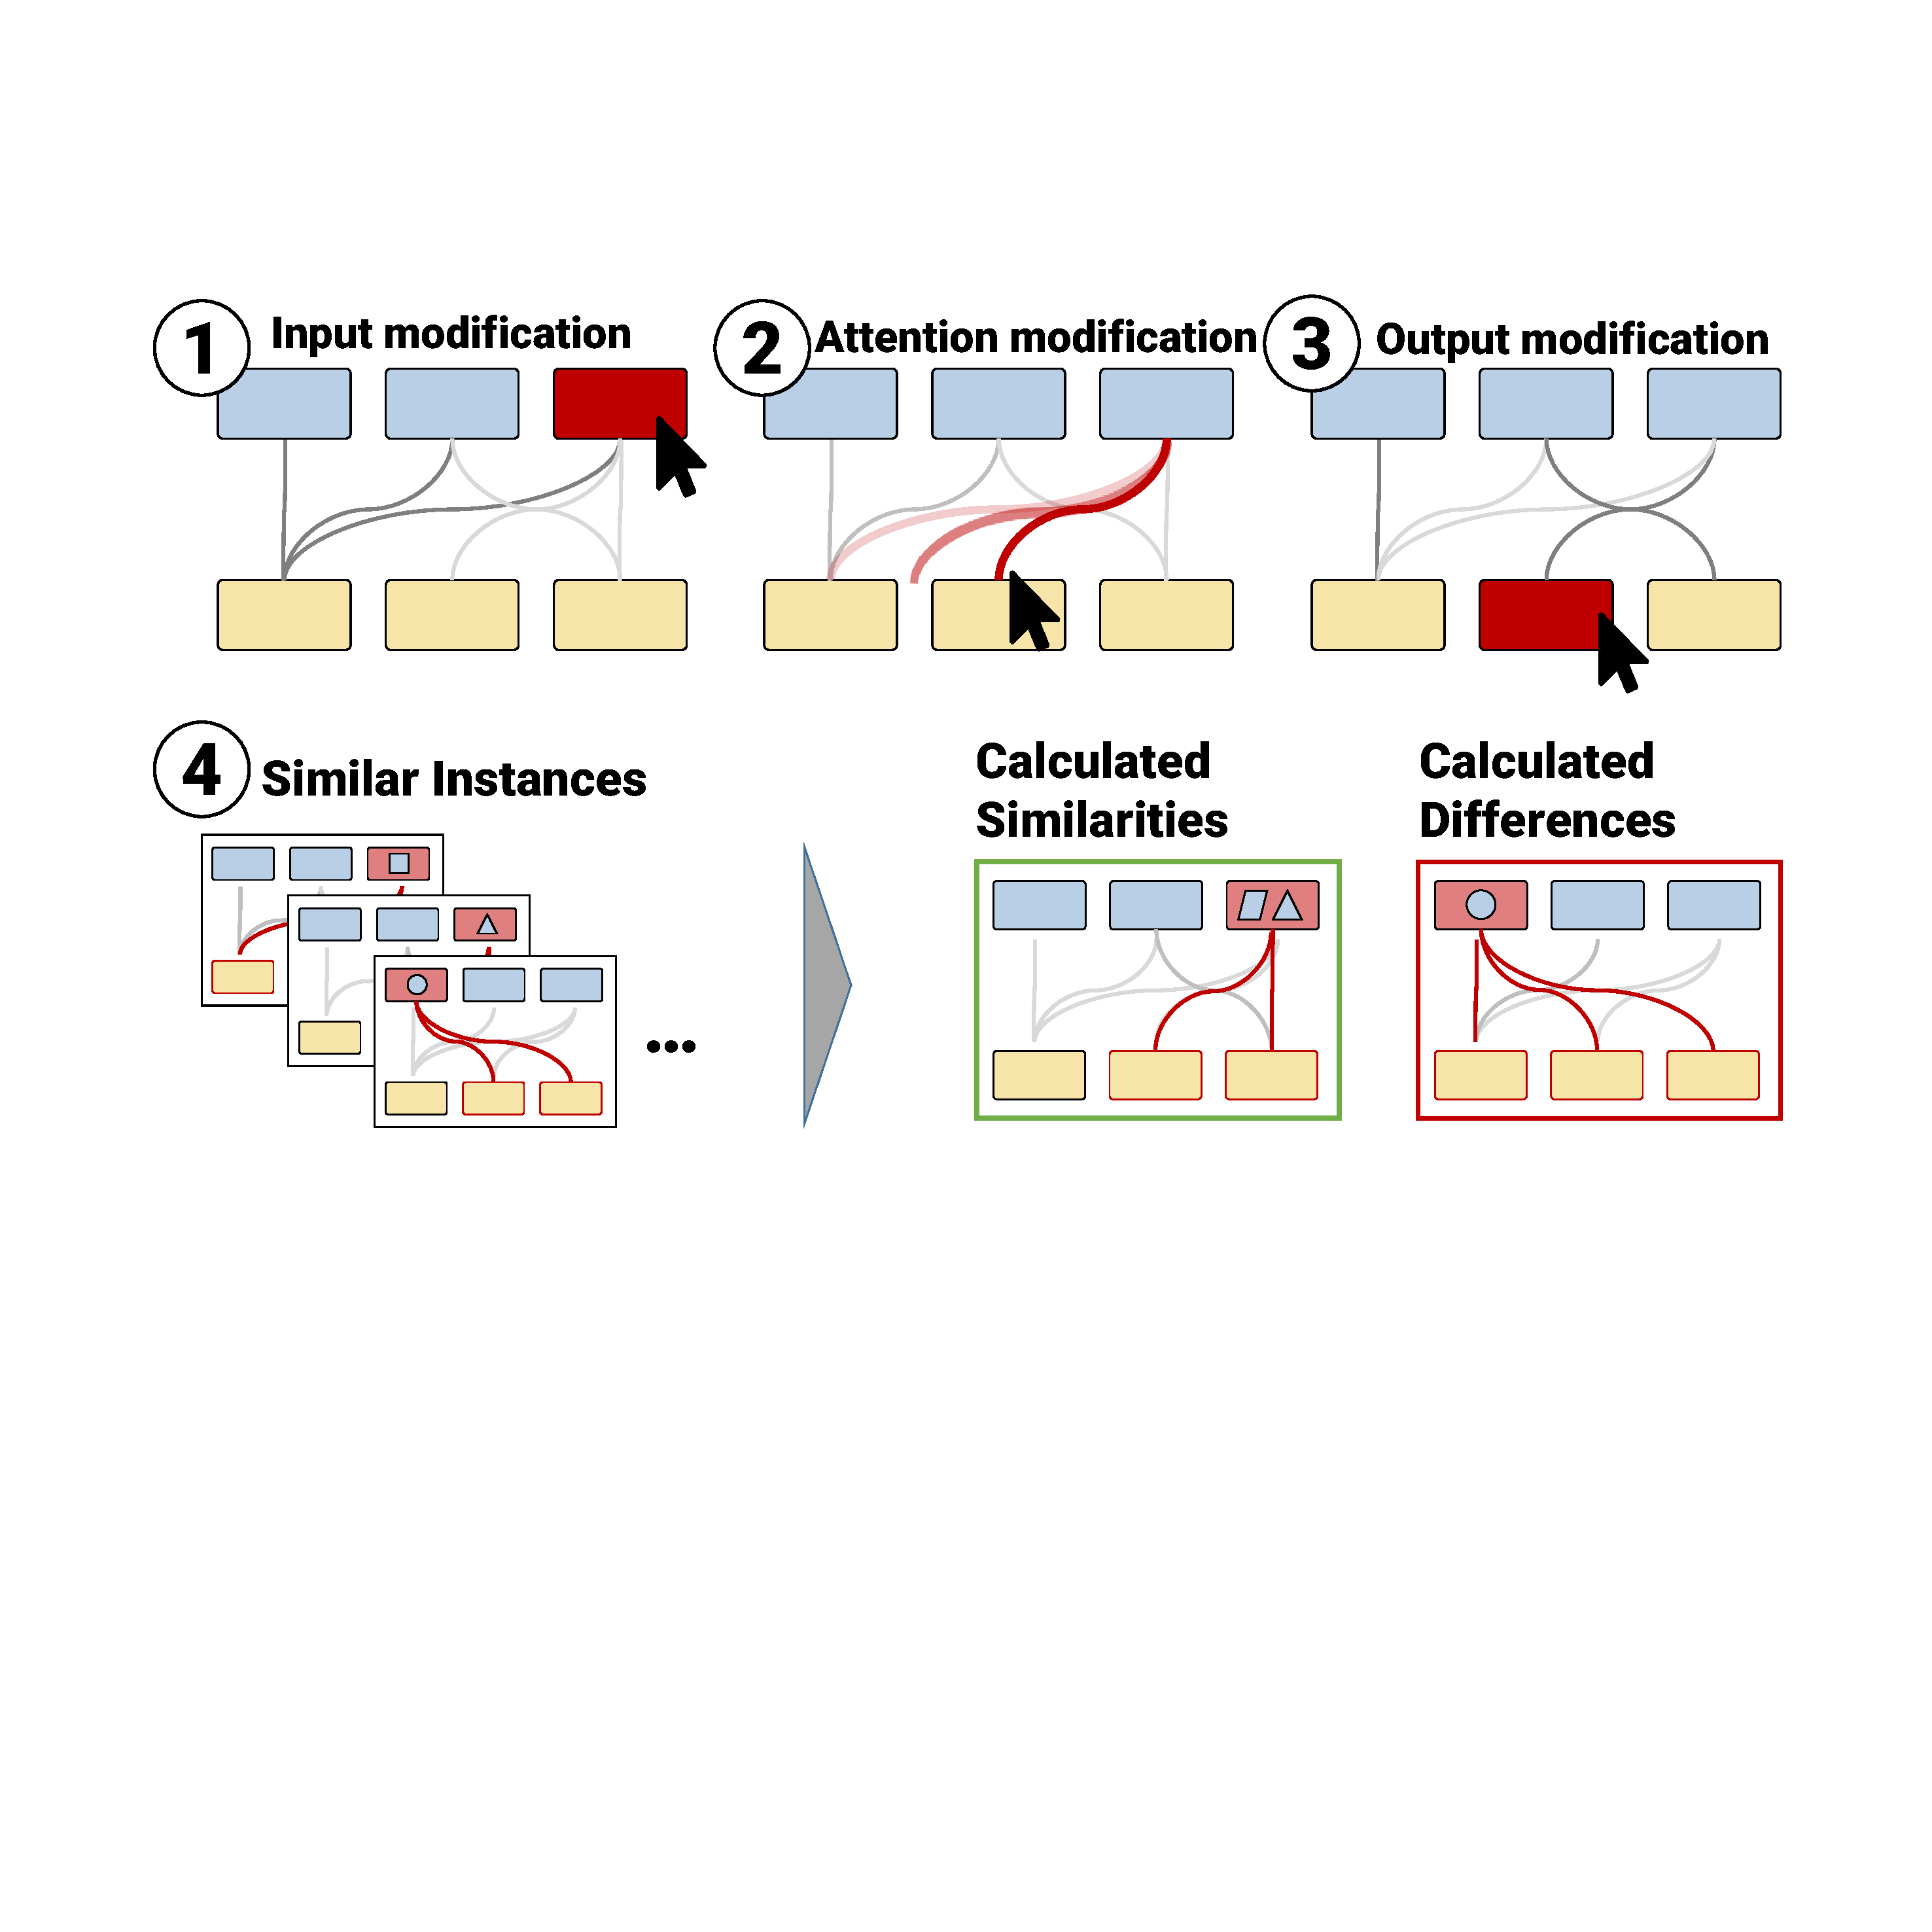
\includegraphics[width=0.7\textwidth]{AttentionVIS}
  \end{center}
\end{frame}


\section{Future}

\begin{frame}{Model}  
  \begin{center}
    \movie[width=\textwidth, repeat, height=0.85\textheight, width=\textwidth, poster, showcontrols]{Temporary}{videos/latnm.mp4}
  \end{center}
\end{frame}

\begin{frame}{Probabilistic Programming}
\begin{center}
  \begin{tikzpicture}
\node[latent] (Y) {$y$};
\node[factor, xshift=1.25cm] (FYS) {$F$};
\node[latent, xshift=2.5cm](S) {$z$};
\node[factor, xshift=3.75cm](FS) {$G$};
\node[xshift=1.25cm, yshift=-0.5cm]() {$T$};
\node[obs, xshift=5cm](X) {$\mathbf{x}$};
\node[obs, xshift=2.5cm, yshift=1.3cm] (A) {$a$};
\node[obs, xshift=2.5cm, yshift=-1.45cm] (L) {$l$};


\plate [inner sep=0.1cm, xshift=0cm, yshift=0.0cm] {t} {(FS)(S)(FYS)} {};
\plate [inner xsep= 0.3cm, inner ysep= 0.2cm, xshift=-0.1cm, yshift=-0.1cm] {a} {(Y)(FYS)(S)(A)(FS)} {};
\plate [inner xsep= 0.3cm, inner ysep= 0.1cm, xshift=0.1cm, yshift=0.2cm] {l} {(Y)(FYS)(S)(L)(FS)} {};
\node[caption, below left=-0.1cm and -0.3cm of a-wrap.north west] {$|\cal{A}|$};
\node[caption, below left=-0.5cm and -0.4cm of l-wrap.south east] {$|\cal{L}|$};

\draw (Y) -- (FYS);
\draw (X) -- (FS);
\draw[-] (X) to [bend left=25] (FYS);
\draw (FYS) -- (S);
\draw (S) -- (FS);
\draw (FS) -- (A);
\draw (FS) -- (L);
\draw[-] (FYS) to [] (A);
\draw[-] (FYS) to [] (L);
\end{tikzpicture}
\end{center}
\end{frame}


\begin{frame}

\end{frame}
